\documentclass[xetex,mathserif,serif]{beamer}
\usepackage{polyglossia}
\setdefaultlanguage[babelshorthands=true]{russian}
\usepackage{minted}
\usepackage{tabu}
\usepackage{moresize}

\useoutertheme{infolines}

\usepackage{fontspec}
\setmainfont{FreeSans}
\newfontfamily{\russianfonttt}{FreeSans}

\definecolor{links}{HTML}{2A1B81}
\hypersetup{colorlinks,linkcolor=,urlcolor=links}

\tabulinesep=1.2mm

\title{Git}
\author[Юрий Литвинов]{Юрий Литвинов\\\small{\textcolor{gray}{yurii.litvinov@gmail.com}}}
\date{23.01.2019г}

\newcommand{\attribution}[1] {
\vspace{-5mm}\begin{flushright}\begin{scriptsize}\textcolor{gray}{\textcopyright\, #1}\end{scriptsize}\end{flushright}
}

\begin{document}

	\frame{\titlepage}

	\section{Домашка}

	\begin{frame}
		\frametitle{Комментарии по домашке}
		\framesubtitle{Концептуальные}
		\begin{itemize}
			\item hashCode() может (и будет) возвращать отрицательные числа, программа должна быть к этому готова
			\item Надо решить, что делать с ключами и значениями null
			\begin{itemize}
				\item Явно запретить и кидать IllegalArgumentException
				\item Разрешить им быть null-ами и придумать другой способ сигнализировать об отсутствии значения
				\item Вообще, null всегда допустим для всех ссылочных типов, поэтому о нём надо помнить
				\begin{itemize}
					\item И иметь юнит-тесты на это!
				\end{itemize}
			\end{itemize}
			\item clear должен ресайзить таблицу обратно до исходного размера, иначе утечка памяти
		\end{itemize}
	\end{frame}

	\begin{frame}
		\frametitle{Комментарии по домашке (2)}
		\framesubtitle{Технические}
		\begin{itemize}
			\item Инициализация полей --- за или против
			\item \mintinline{java}|@BeforeEach| для инициализации хеш-таблицы в тестах
			\item Если тип переменной очевиден из правой части --- var
			\item Сдавать решение одним коммитом немудро
		\end{itemize}
	\end{frame}

	\begin{frame}
		\frametitle{Комментарии по домашке (3)}
		\framesubtitle{По оформлению}
		\begin{itemize}
			\item Комментарии не должны начинаться с \mintinline{java}|@return|
			\item Не надо сокращать идентификаторы
			\item Стоит избегать побочных эффектов в выражениях
			\item Каждый класс (не вложенный) должен быть в своём файле
		\end{itemize}
	\end{frame}

	\section{Git}

	\begin{frame}
		\frametitle{Git}
		\begin{columns}
			\begin{column}{0.5\textwidth}
				\begin{itemize}
					\item Не GitHub!
					\item Не файлообменник
					\item Распределённая система контроля версий
					\item Удобная поддержка веток
				\end{itemize}
			\end{column}
			\begin{column}{0.5\textwidth}
				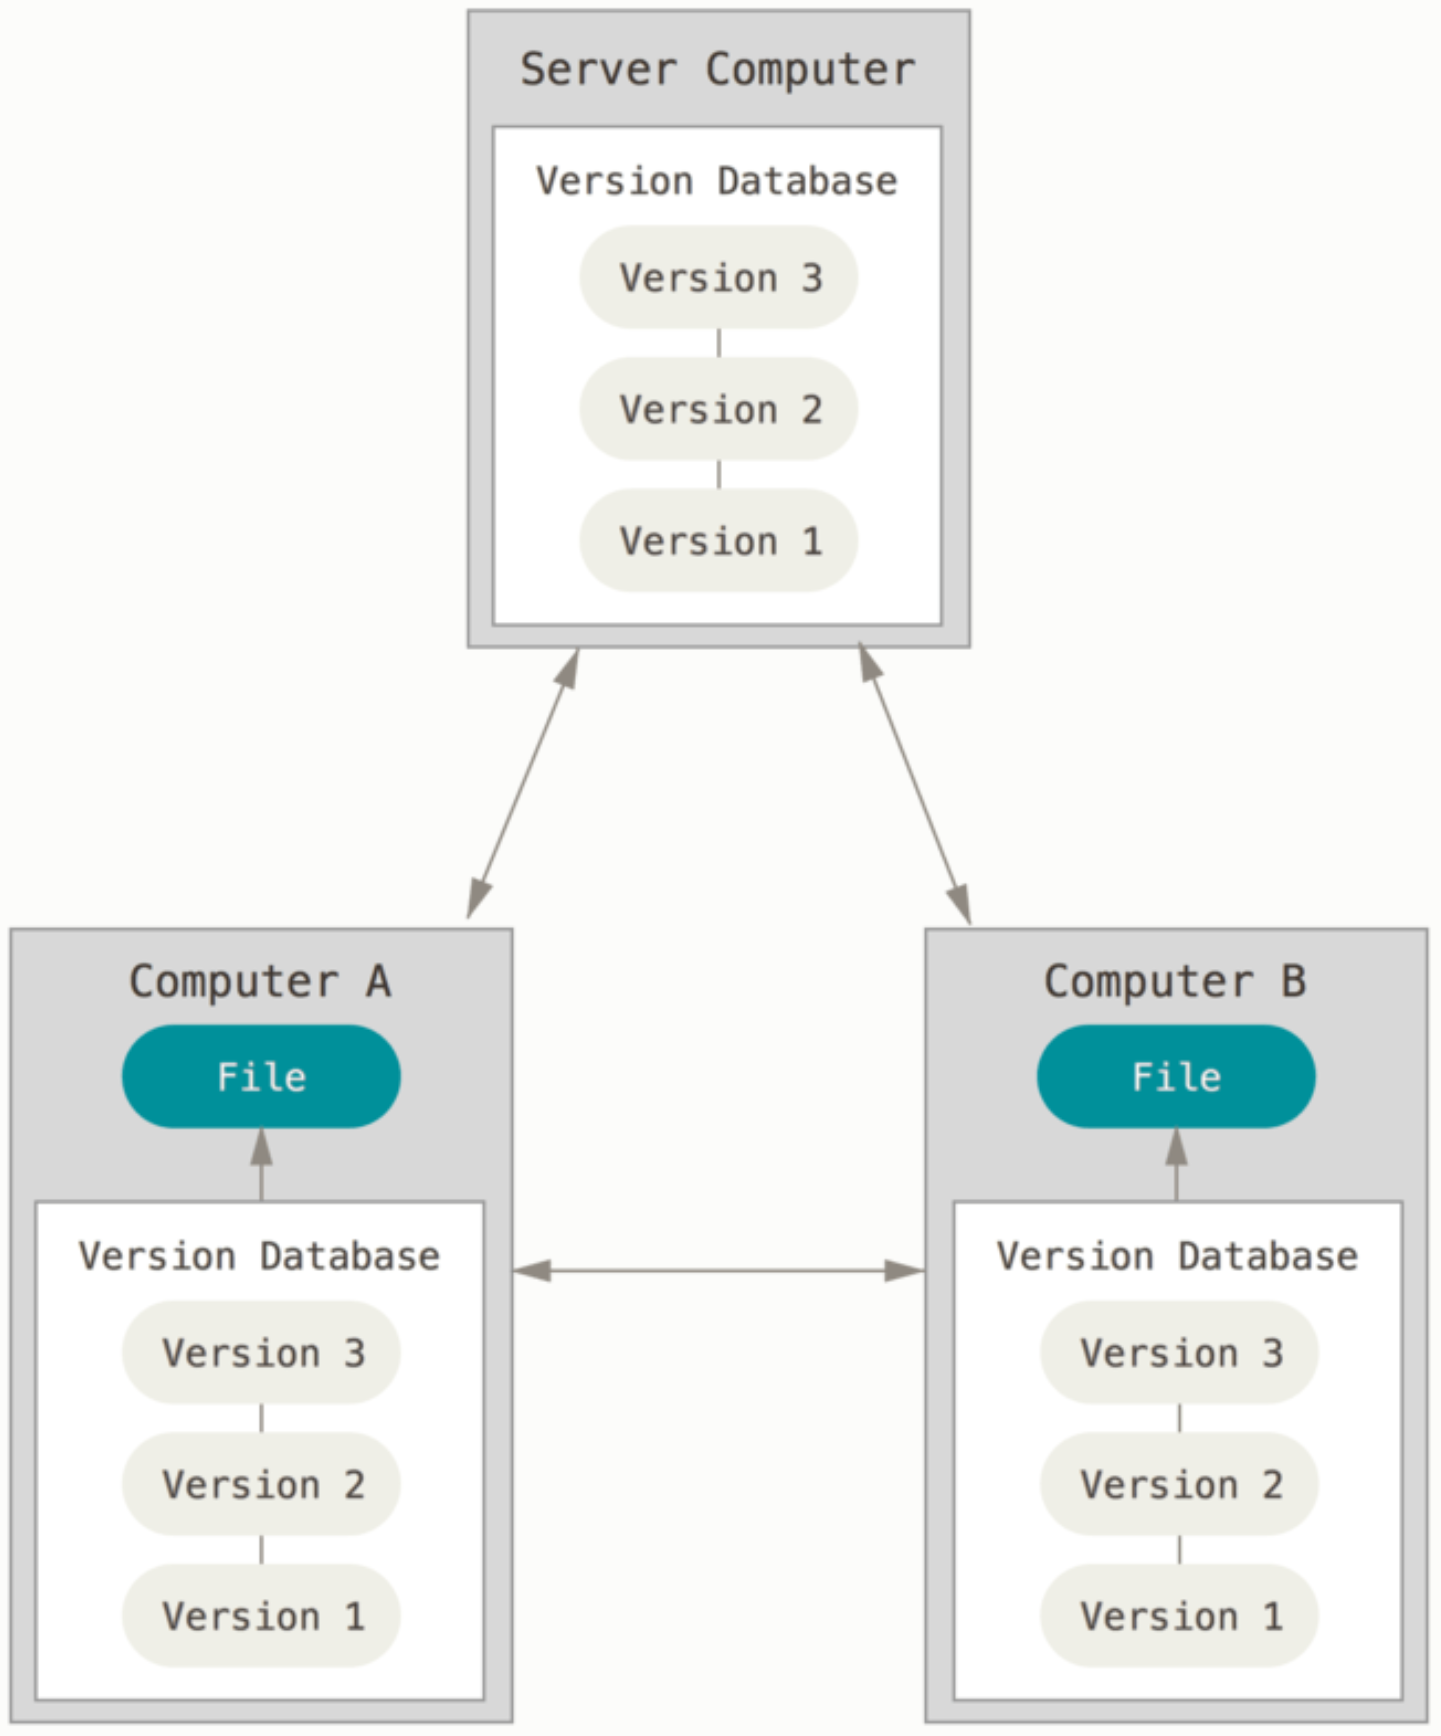
\includegraphics[width=0.9\textwidth]{distributedVcs.png}
			\end{column}
		\end{columns}
	\end{frame}

	\begin{frame}
		\frametitle{Управление версиями}
		\begin{center}
			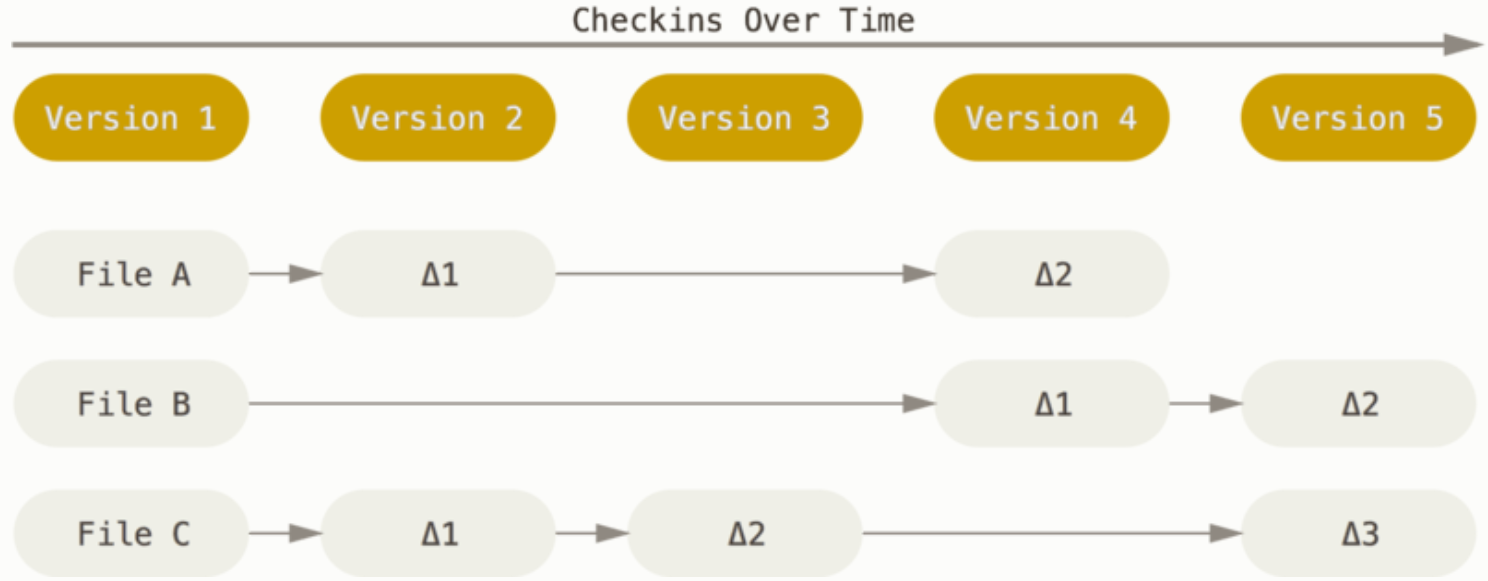
\includegraphics[width=0.6\textwidth]{deltaVersioning.png}

			\vspace{5mm}
			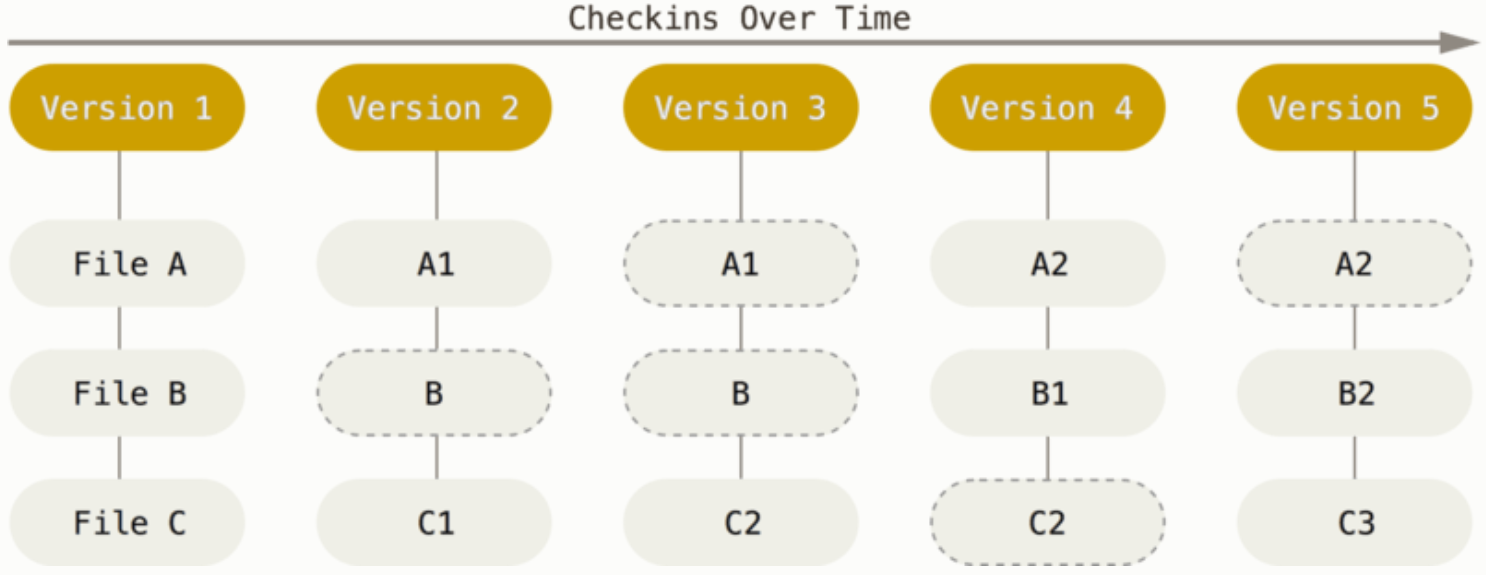
\includegraphics[width=0.6\textwidth]{snapshotVersioning.png}
			\attribution{https://git-scm.com/book/ru}
		\end{center}
	\end{frame}

	\begin{frame}
		\frametitle{Дельта}
		\begin{center}
			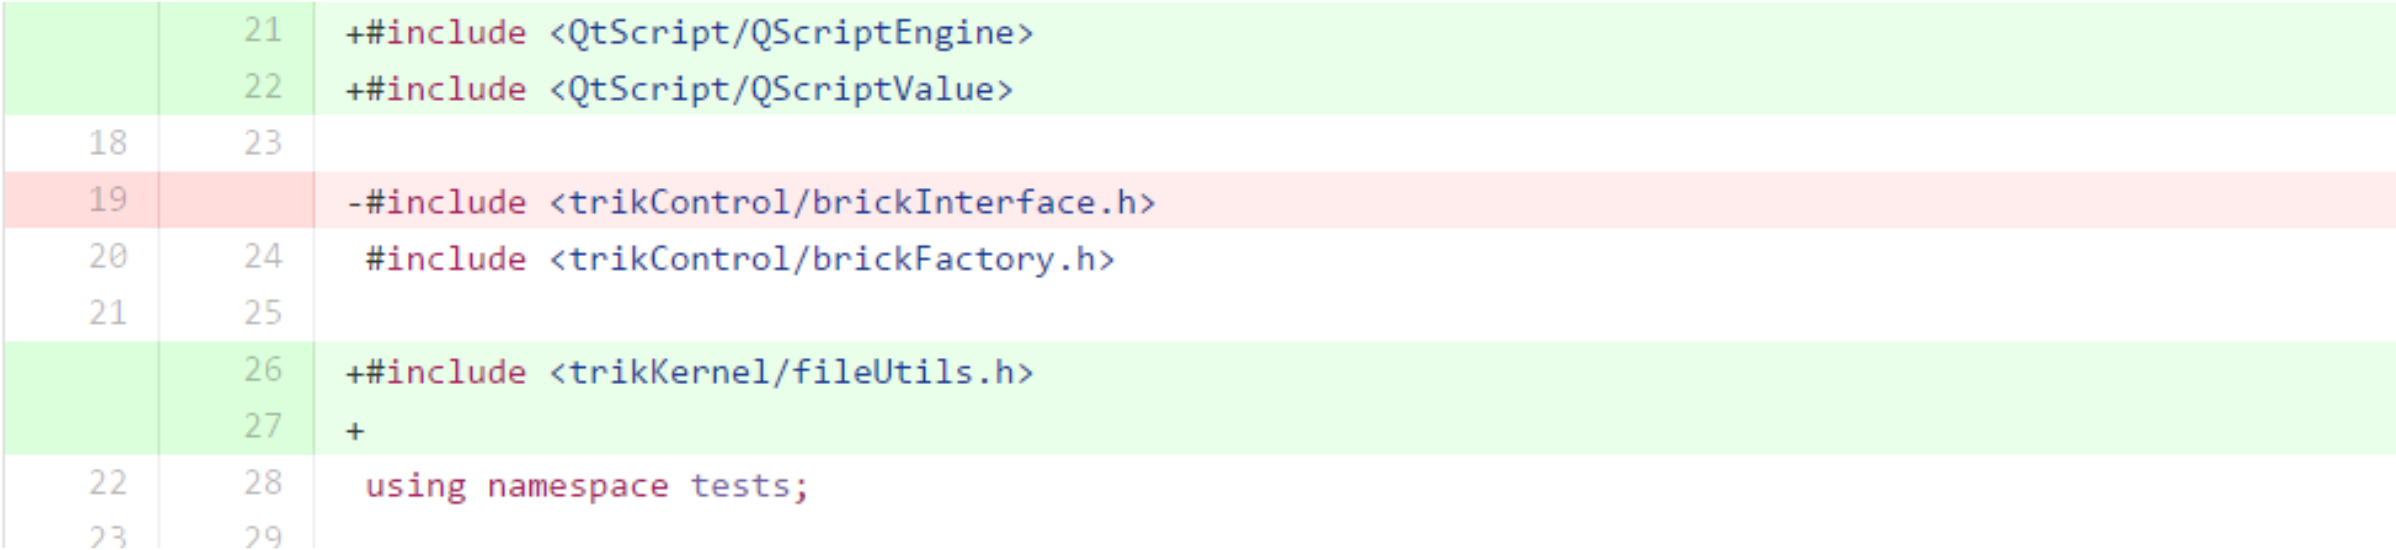
\includegraphics[width=0.8\textwidth]{delta.png}
		\end{center}
	\end{frame}

	\begin{frame}
		\frametitle{Жизненный цикл файла}
		\begin{center}
			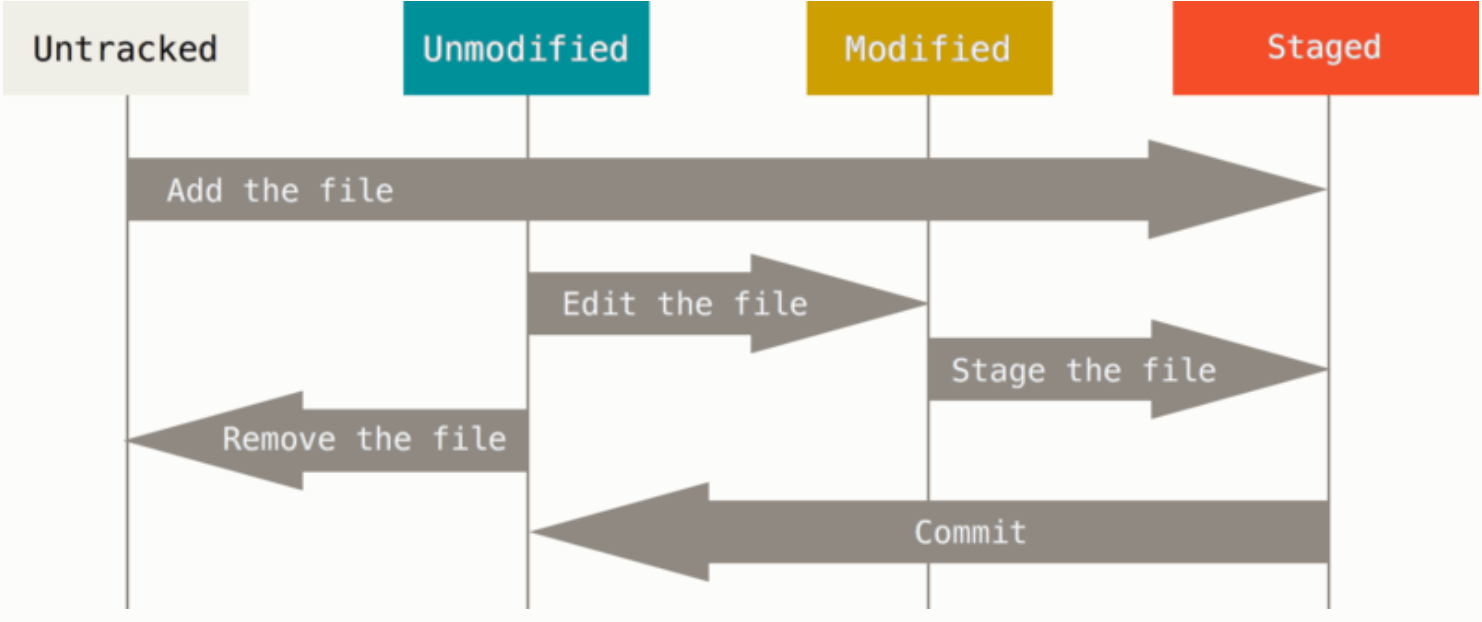
\includegraphics[width=0.8\textwidth]{fileLifeCycle.png}
			\attribution{https://git-scm.com/book/ru}
		\end{center}
	\end{frame}

	\begin{frame}
		\frametitle{Основные команды}
		\begin{itemize}
			\item git add --- добавить новый файл под управление git или добавить изменение к коммиту
			\item git status --- показать список изменённых/добавленных/удалённых файлов
			\item git diff --- показать изменения по каждому файлу
			\item git commit --- зафиксировать изменения, создав новый коммит
			\item git rm --- удалить файл и удалить его из репозиторий
			\item git log --- просмотреть список коммитов
			\item git checkout --- откатить изменения в файле или перейти на другую ветку
		\end{itemize}
	\end{frame}

	\begin{frame}
		\frametitle{Удалённые репозитории}
		\begin{columns}
			\begin{column}{0.4\textwidth}
				\begin{itemize}
					\item git clone
					\item git remote
					\item git push
					\item git fetch
					\item git pull
				\end{itemize}
			\end{column}
			\begin{column}{0.6\textwidth}
				\begin{center}
					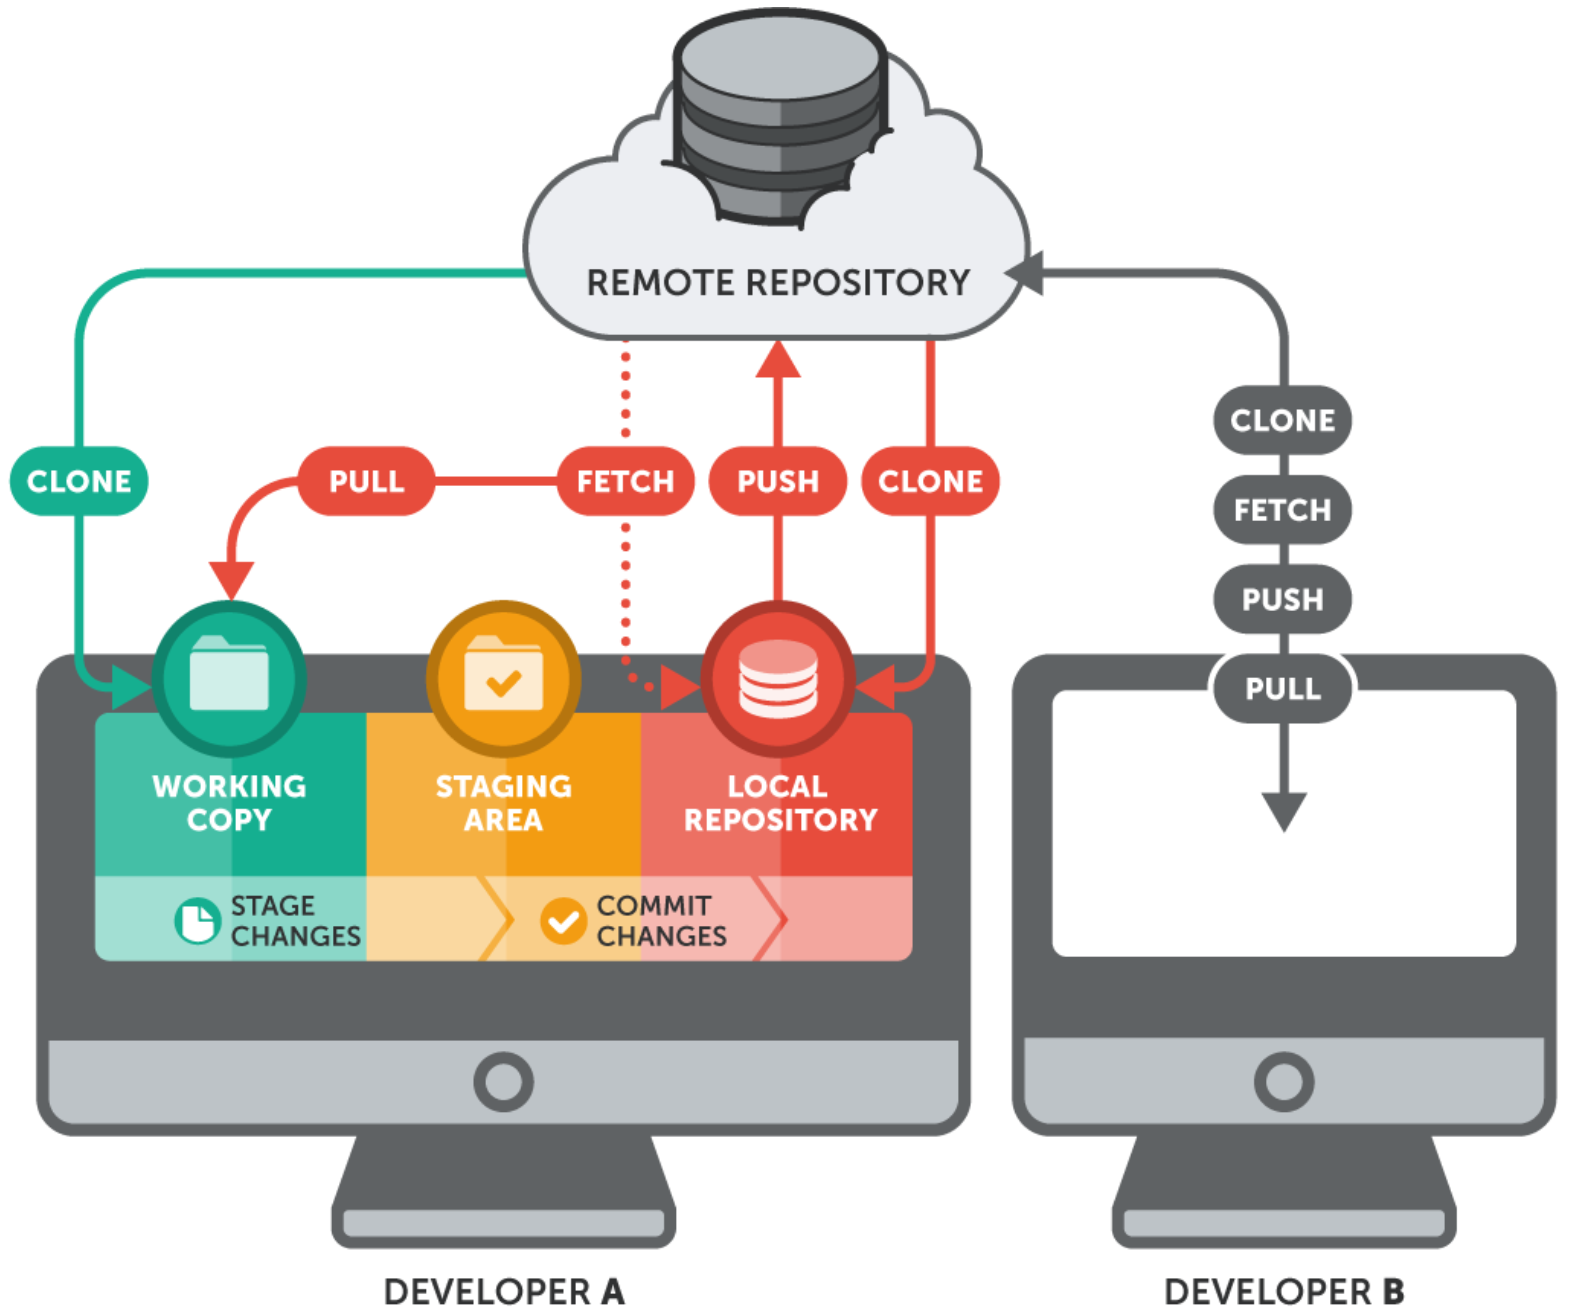
\includegraphics[width=0.95\textwidth]{remoteRepos.png}
					\attribution{https://www.git-tower.com/learn/git/ebook/en}
				\end{center}
			\end{column}
		\end{columns}
	\end{frame}

	\begin{frame}[fragile]
		\frametitle{Как всё устроено}
		\begin{minted}{text}
$ git add README test.rb LICENSE
$ git commit -m 'initial commit of my project'
		\end{minted}
		\begin{center}
			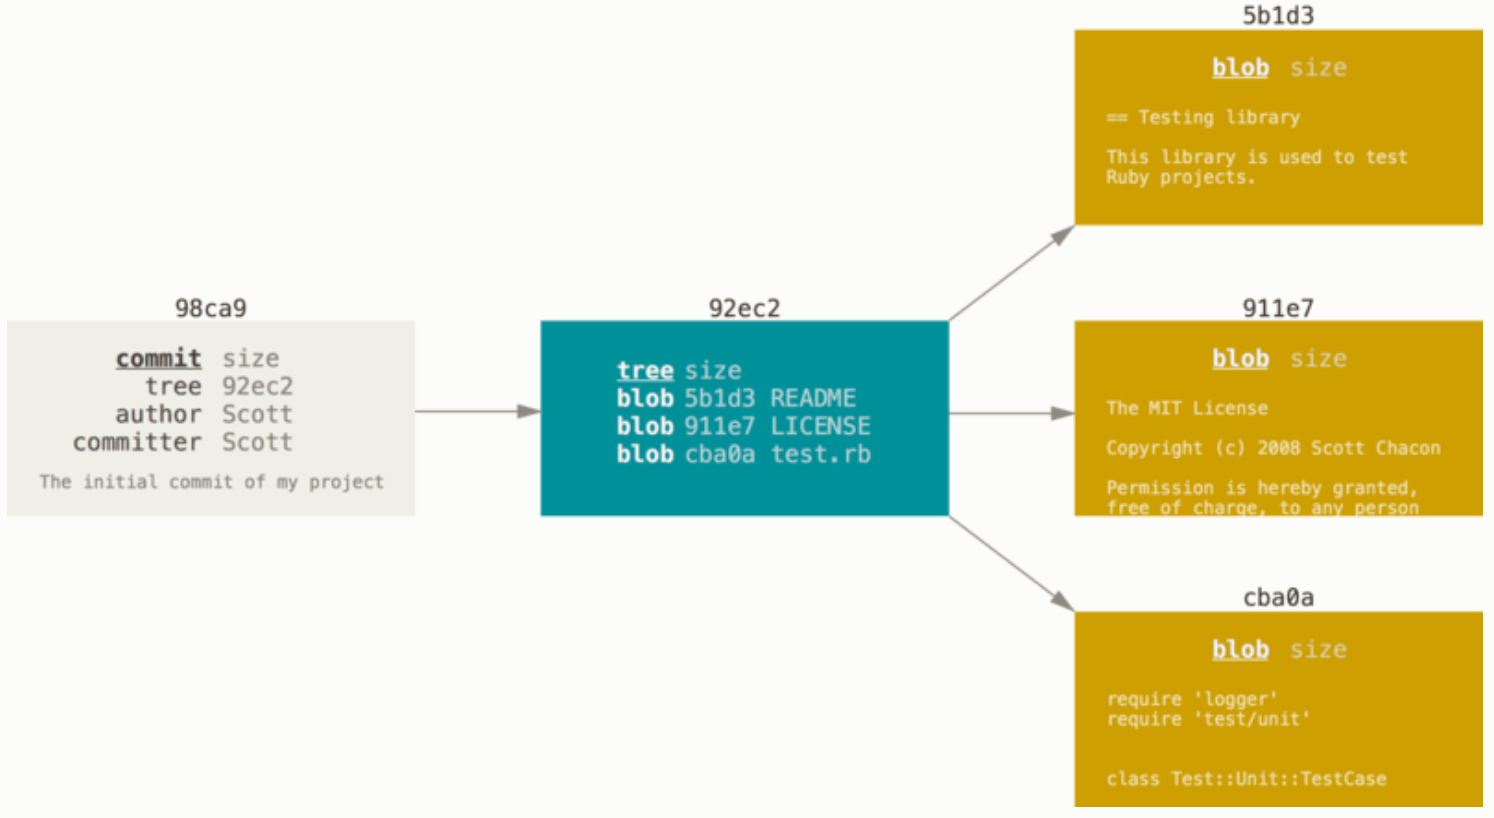
\includegraphics[width=0.8\textwidth]{blobs.png}
			\attribution{https://git-scm.com/book/ru}
		\end{center}
	\end{frame}

	\begin{frame}
		\frametitle{Коммит и его родители}
		\begin{center}
			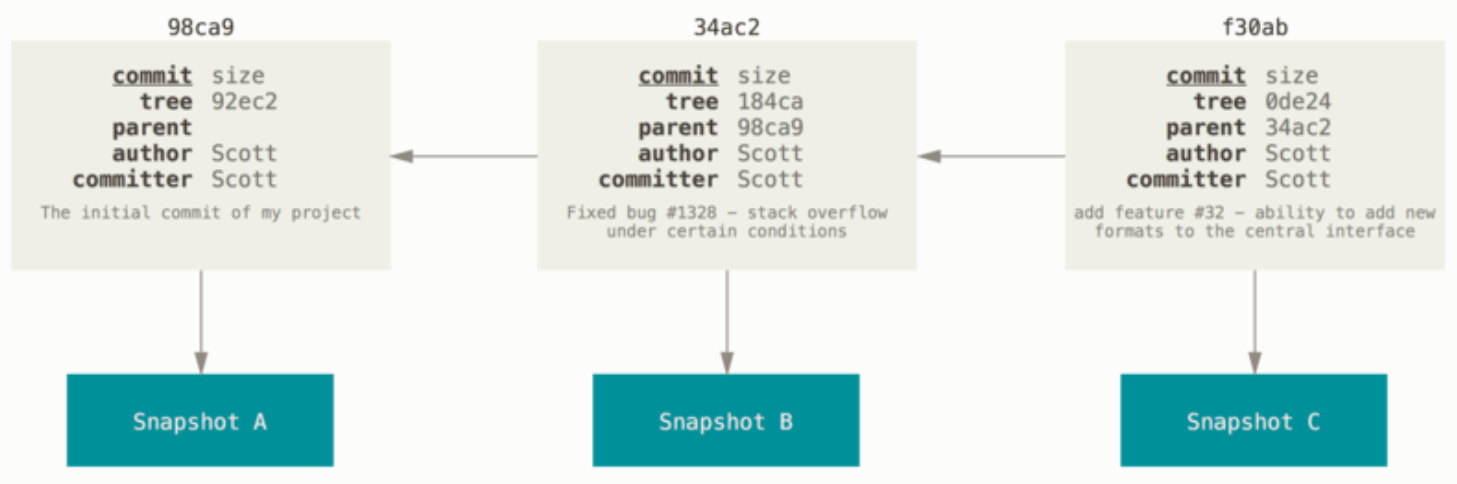
\includegraphics[width=0.8\textwidth]{commits.png}
			\attribution{https://git-scm.com/book/ru}
		\end{center}
	\end{frame}

	\begin{frame}
		\frametitle{Ветки}
		\begin{center}
			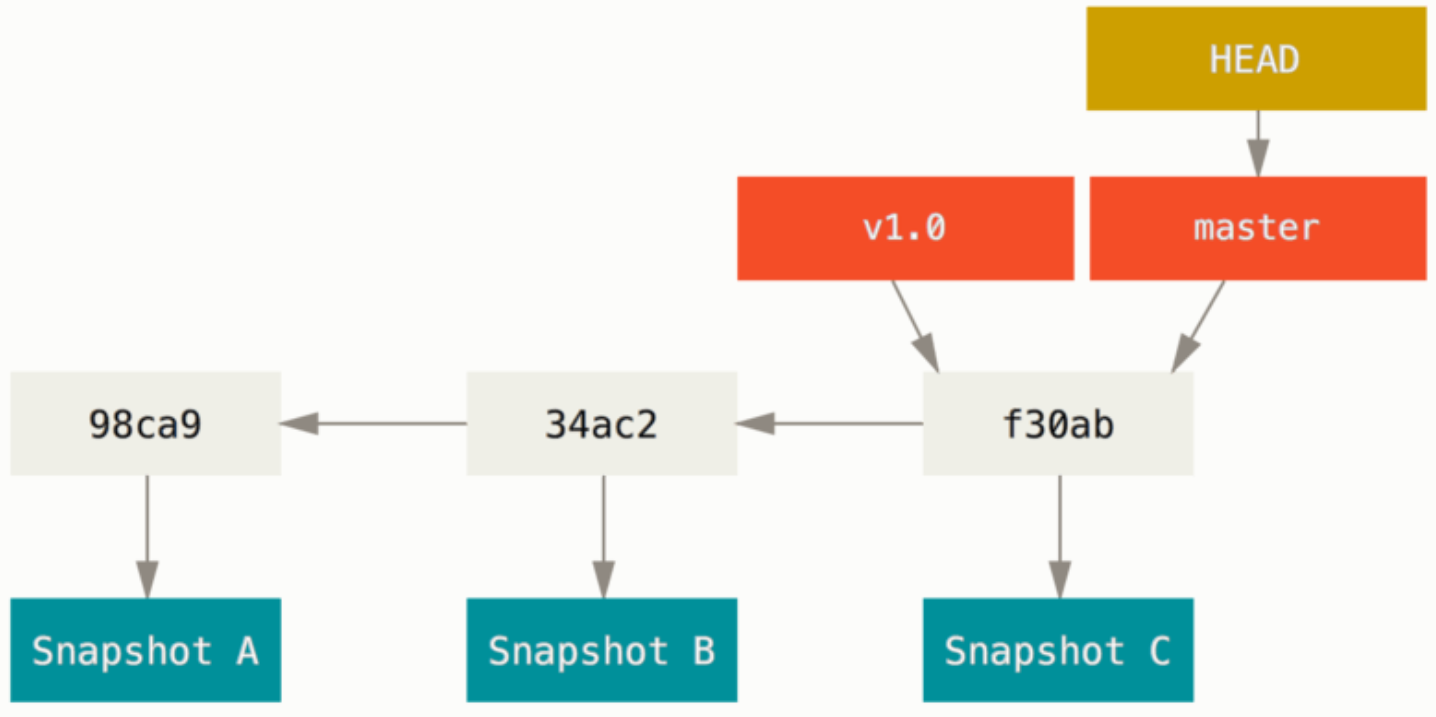
\includegraphics[width=0.8\textwidth]{branches.png}
			\attribution{https://git-scm.com/book/ru}
		\end{center}
	\end{frame}

	\begin{frame}
		\frametitle{Ссылки, как это выглядит}
		\begin{center}
			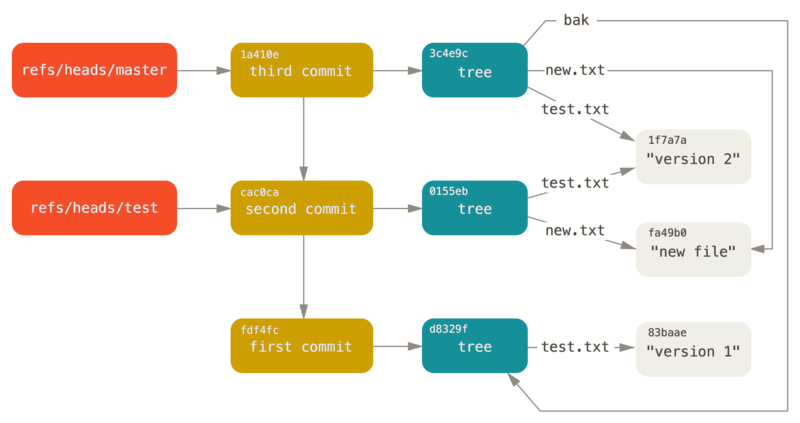
\includegraphics[width=0.9\textwidth]{gitRefs.png}
		\end{center}
	\end{frame}

	\begin{frame}[fragile]
		\frametitle{HEAD}
		Теперь не надо помнить хеши, но как переключаться между ветками?

		Текущая ветка хранится в HEAD. HEAD --- символическая ссылка, то есть ссылка на другую ссылку.
		\begin{minted}{text}
$ cat .git/HEAD
ref: refs/heads/master
		\end{minted}
	\end{frame}

	\begin{frame}[fragile]
		\frametitle{Создание ветки}
		\begin{minted}{text}
$ git branch testing
		\end{minted}
		\begin{center}
			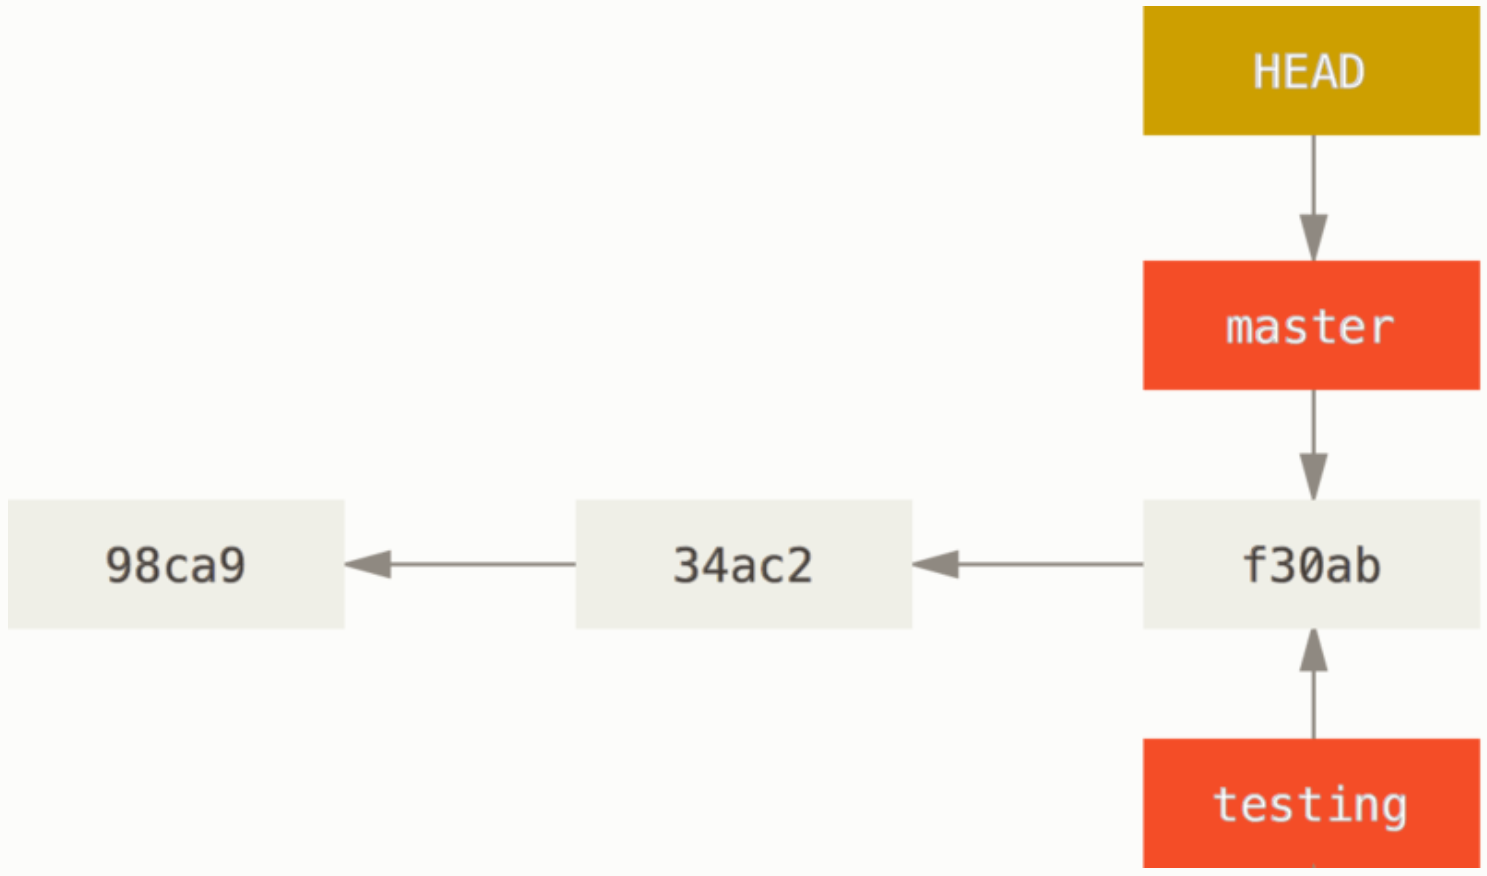
\includegraphics[width=0.8\textwidth]{creatingBranch.png}
			\attribution{https://git-scm.com/book/ru}
		\end{center}
	\end{frame}

	\begin{frame}[fragile]
		\frametitle{Переключение ветки}
		\begin{minted}{text}
$ git checkout testing
		\end{minted}
		\begin{center}
			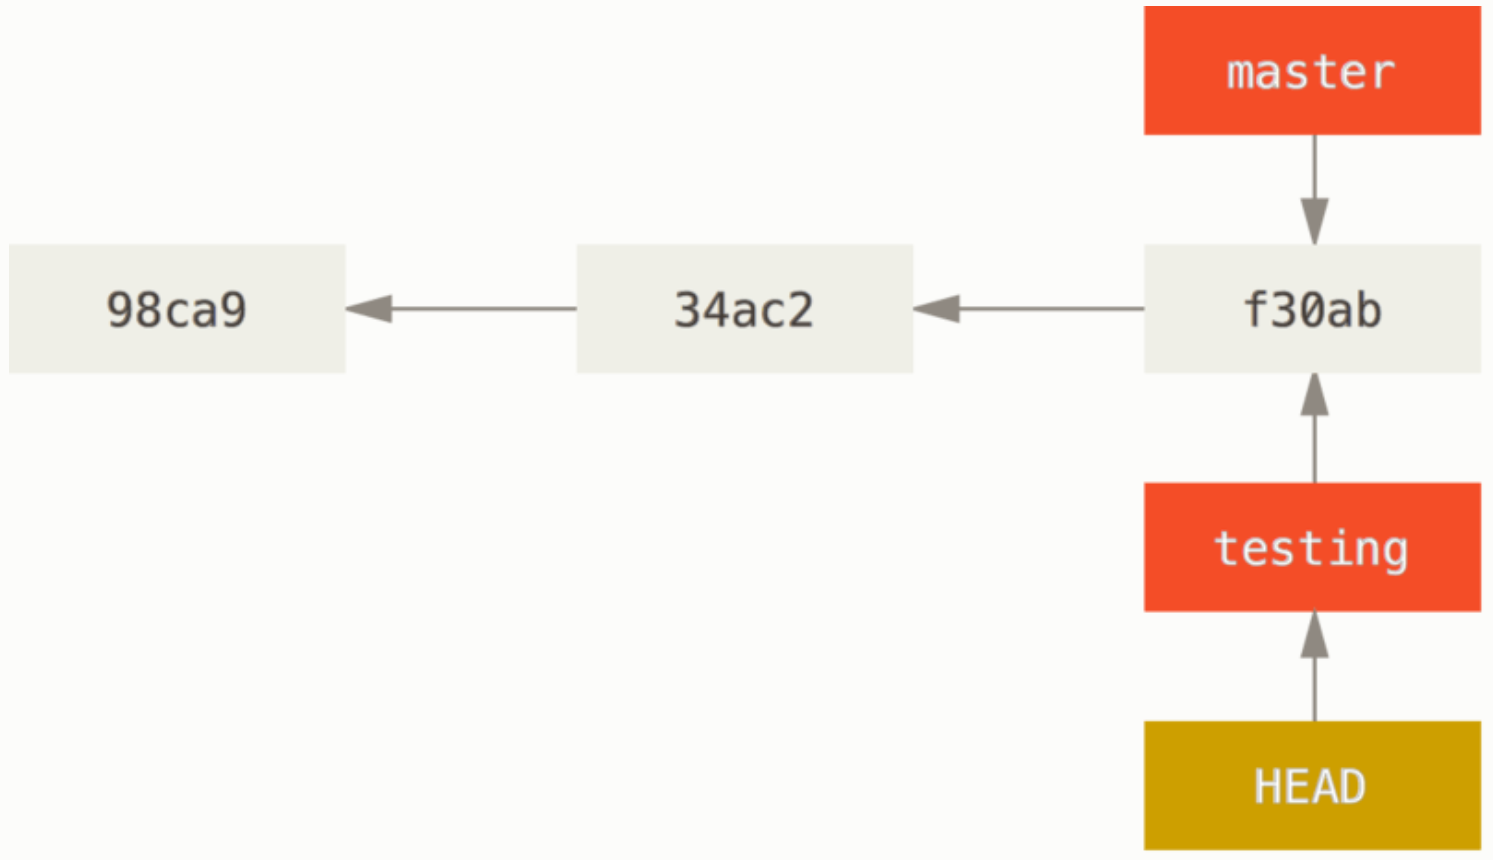
\includegraphics[width=0.8\textwidth]{checkout.png}
			\attribution{https://git-scm.com/book/ru}
		\end{center}
	\end{frame}

	\begin{frame}[fragile]
		\frametitle{Новый коммит}
		\begin{minted}{text}
<Что-то поделали с файлами в рабочей копии>
$ git add <изменения, которые хотим коммитить>
$ git commit -m 'made a change'
		\end{minted}
		\begin{center}
			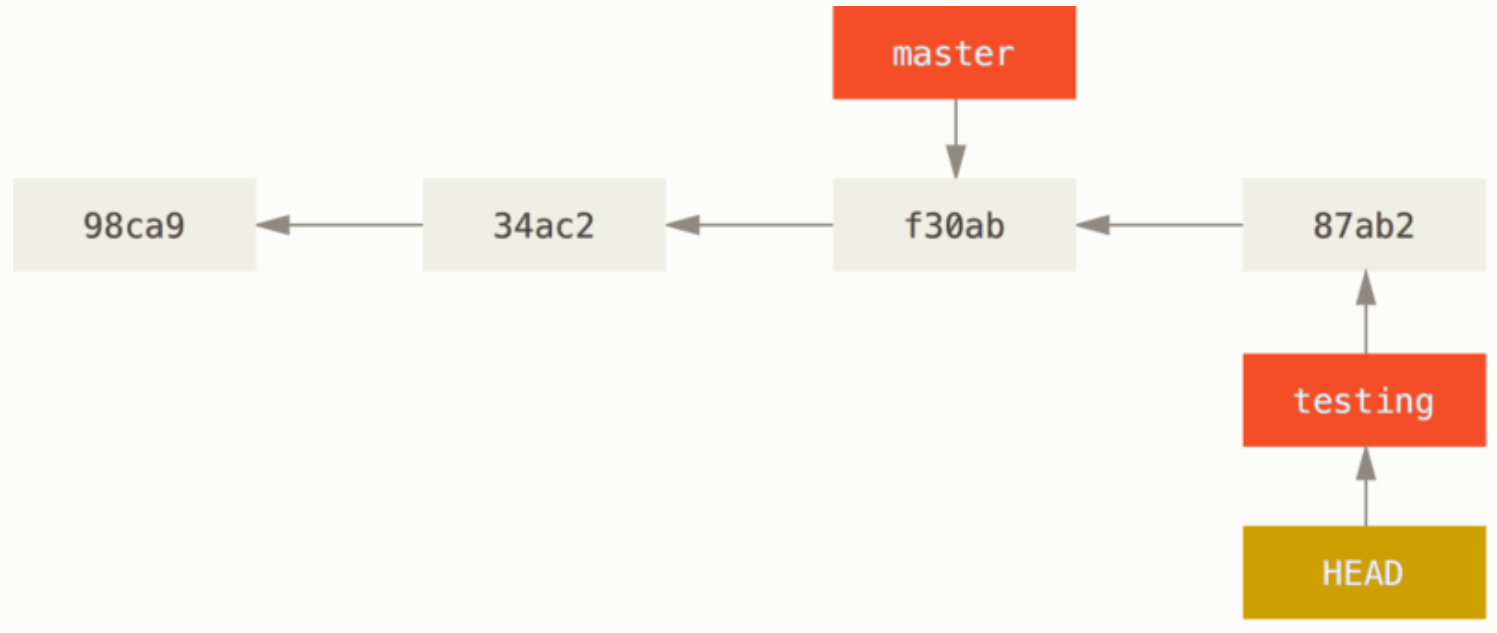
\includegraphics[width=0.8\textwidth]{newCommit.png}
			\attribution{https://git-scm.com/book/ru}
		\end{center}
	\end{frame}

	\begin{frame}[fragile]
		\frametitle{Переключимся на master}
		\begin{minted}{text}
$ git checkout master
		\end{minted}
		\begin{center}
			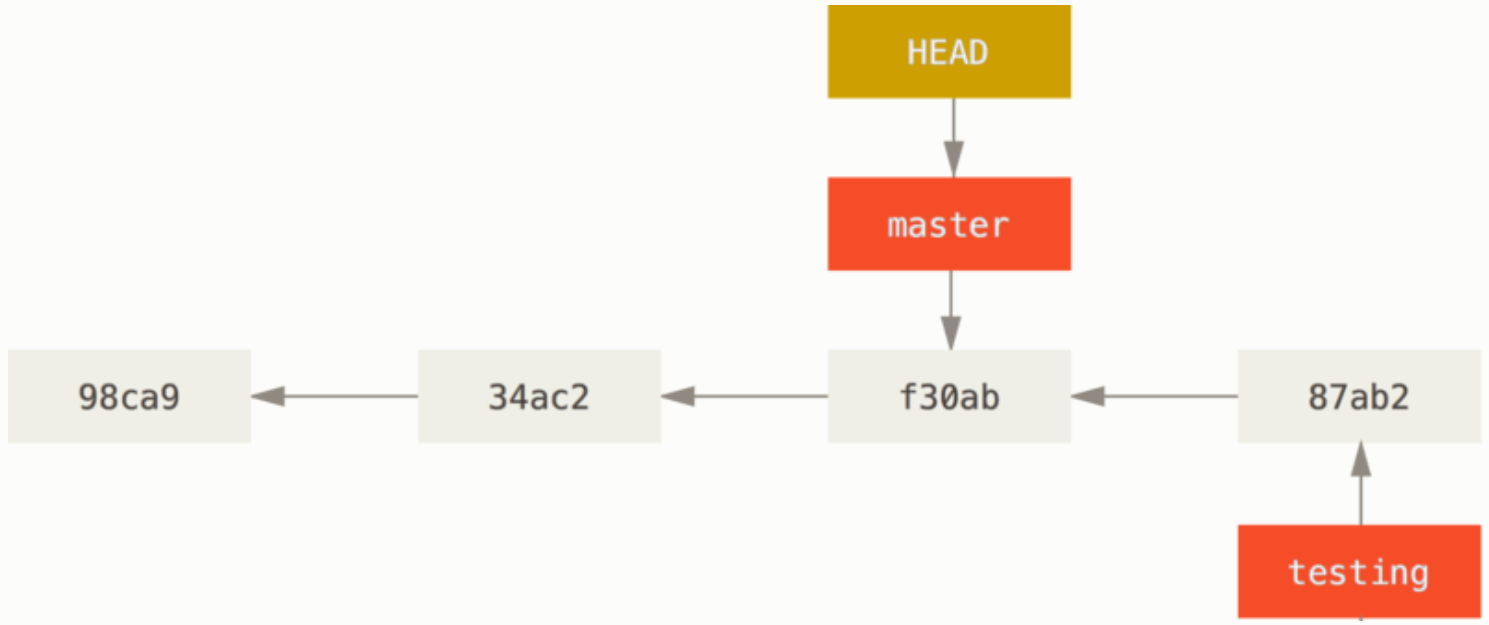
\includegraphics[width=0.8\textwidth]{checkoutToMaster.png}
			\attribution{https://git-scm.com/book/ru}
		\end{center}
	\end{frame}

	\begin{frame}[fragile]
		\frametitle{Сделаем новый коммит там}
		\begin{minted}{text}
<Что-то поделали с файлами в рабочей копии>
$ git add <изменения, которые хотим коммитить>
$ git commit -m 'made other changes'
		\end{minted}
		\begin{center}
			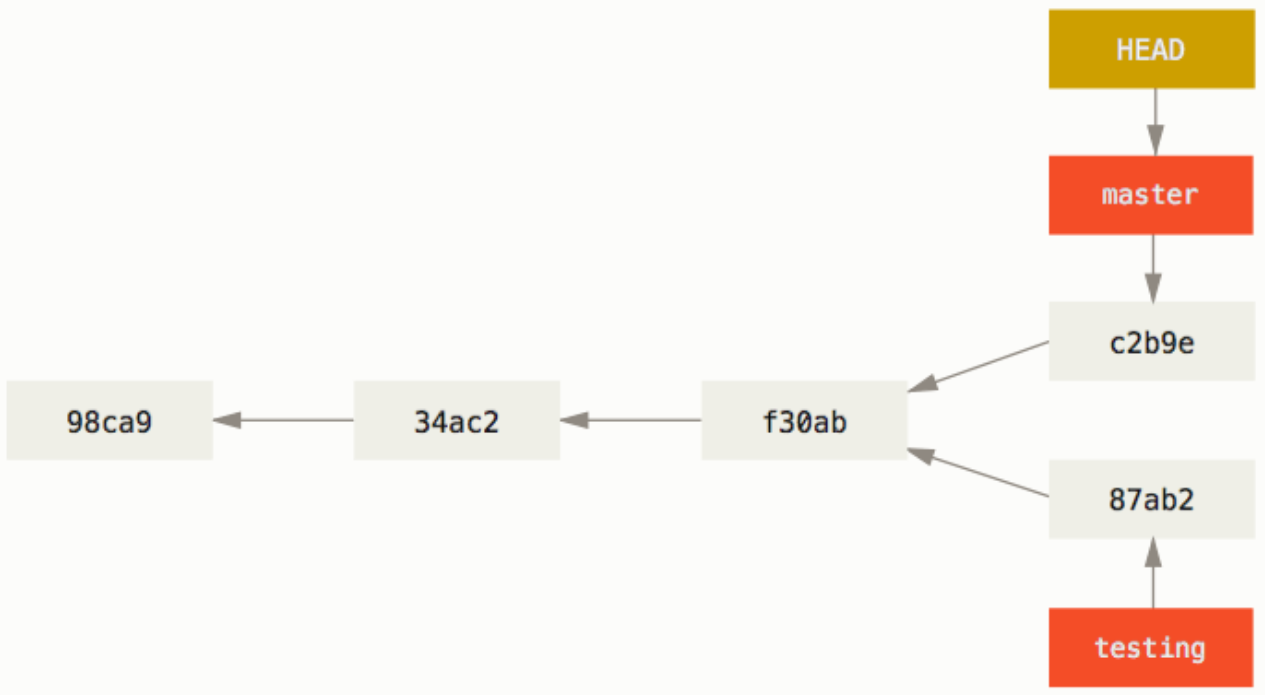
\includegraphics[width=0.8\textwidth]{newCommitToMaster.png}
			\attribution{https://git-scm.com/book/ru}
		\end{center}
	\end{frame}

	\begin{frame}[fragile]
		\frametitle{Слияние веток}
		\begin{minted}{text}
$ git checkout master
Switched to branch 'master'
$ git merge testing
Merge made by the 'recursive' strategy.
index.html |    1 +
1 file changed, 1 insertion(+)
		\end{minted}
		\begin{center}
			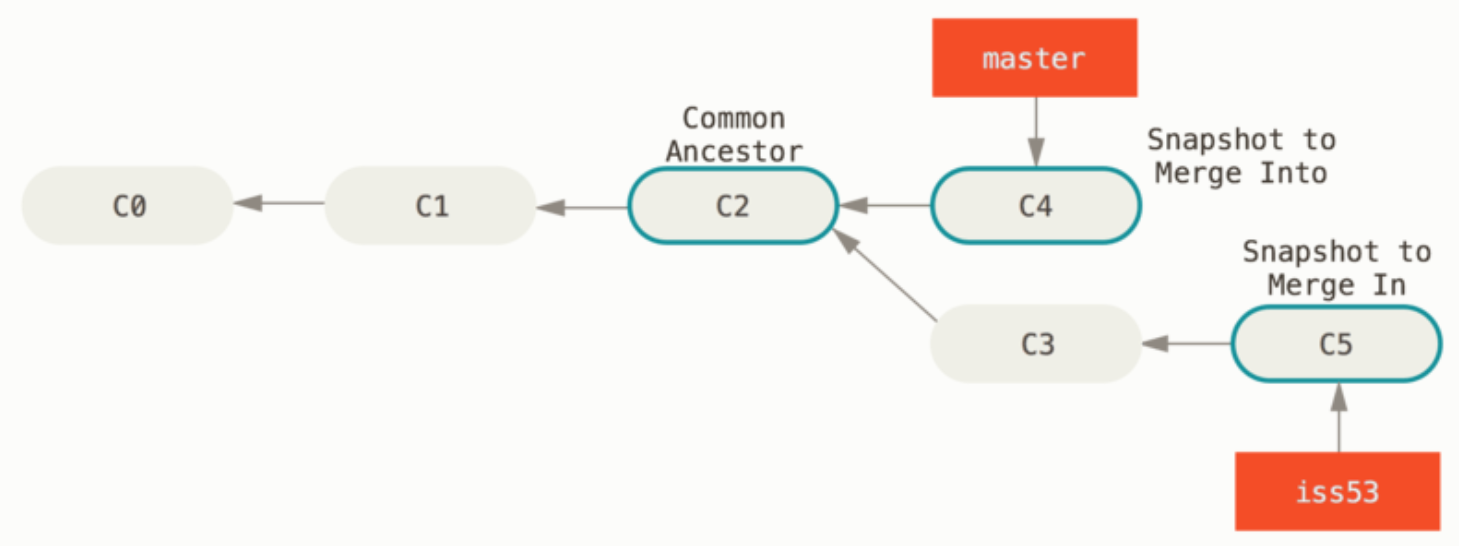
\includegraphics[width=0.8\textwidth]{merge.png}
			\attribution{https://git-scm.com/book/ru}
		\end{center}
	\end{frame}

	\begin{frame}
		\frametitle{Результат}
		\begin{center}
			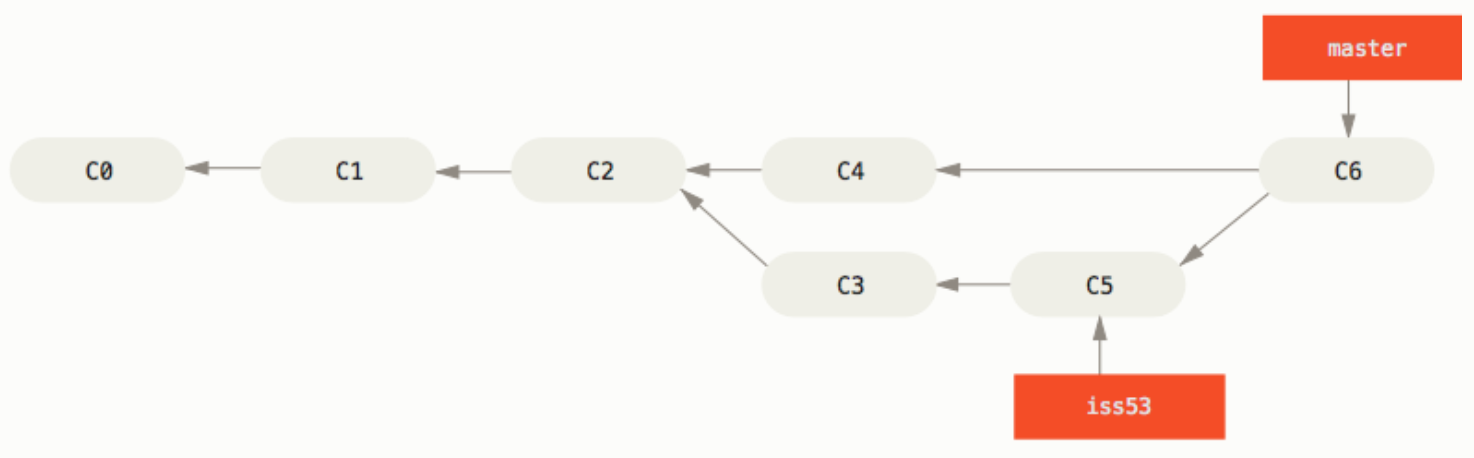
\includegraphics[width=0.8\textwidth]{mergeResult.png}
			\attribution{https://git-scm.com/book/ru}
		\end{center}
	\end{frame}

	\begin{frame}
		\frametitle{Конфликты}
		\begin{center}
			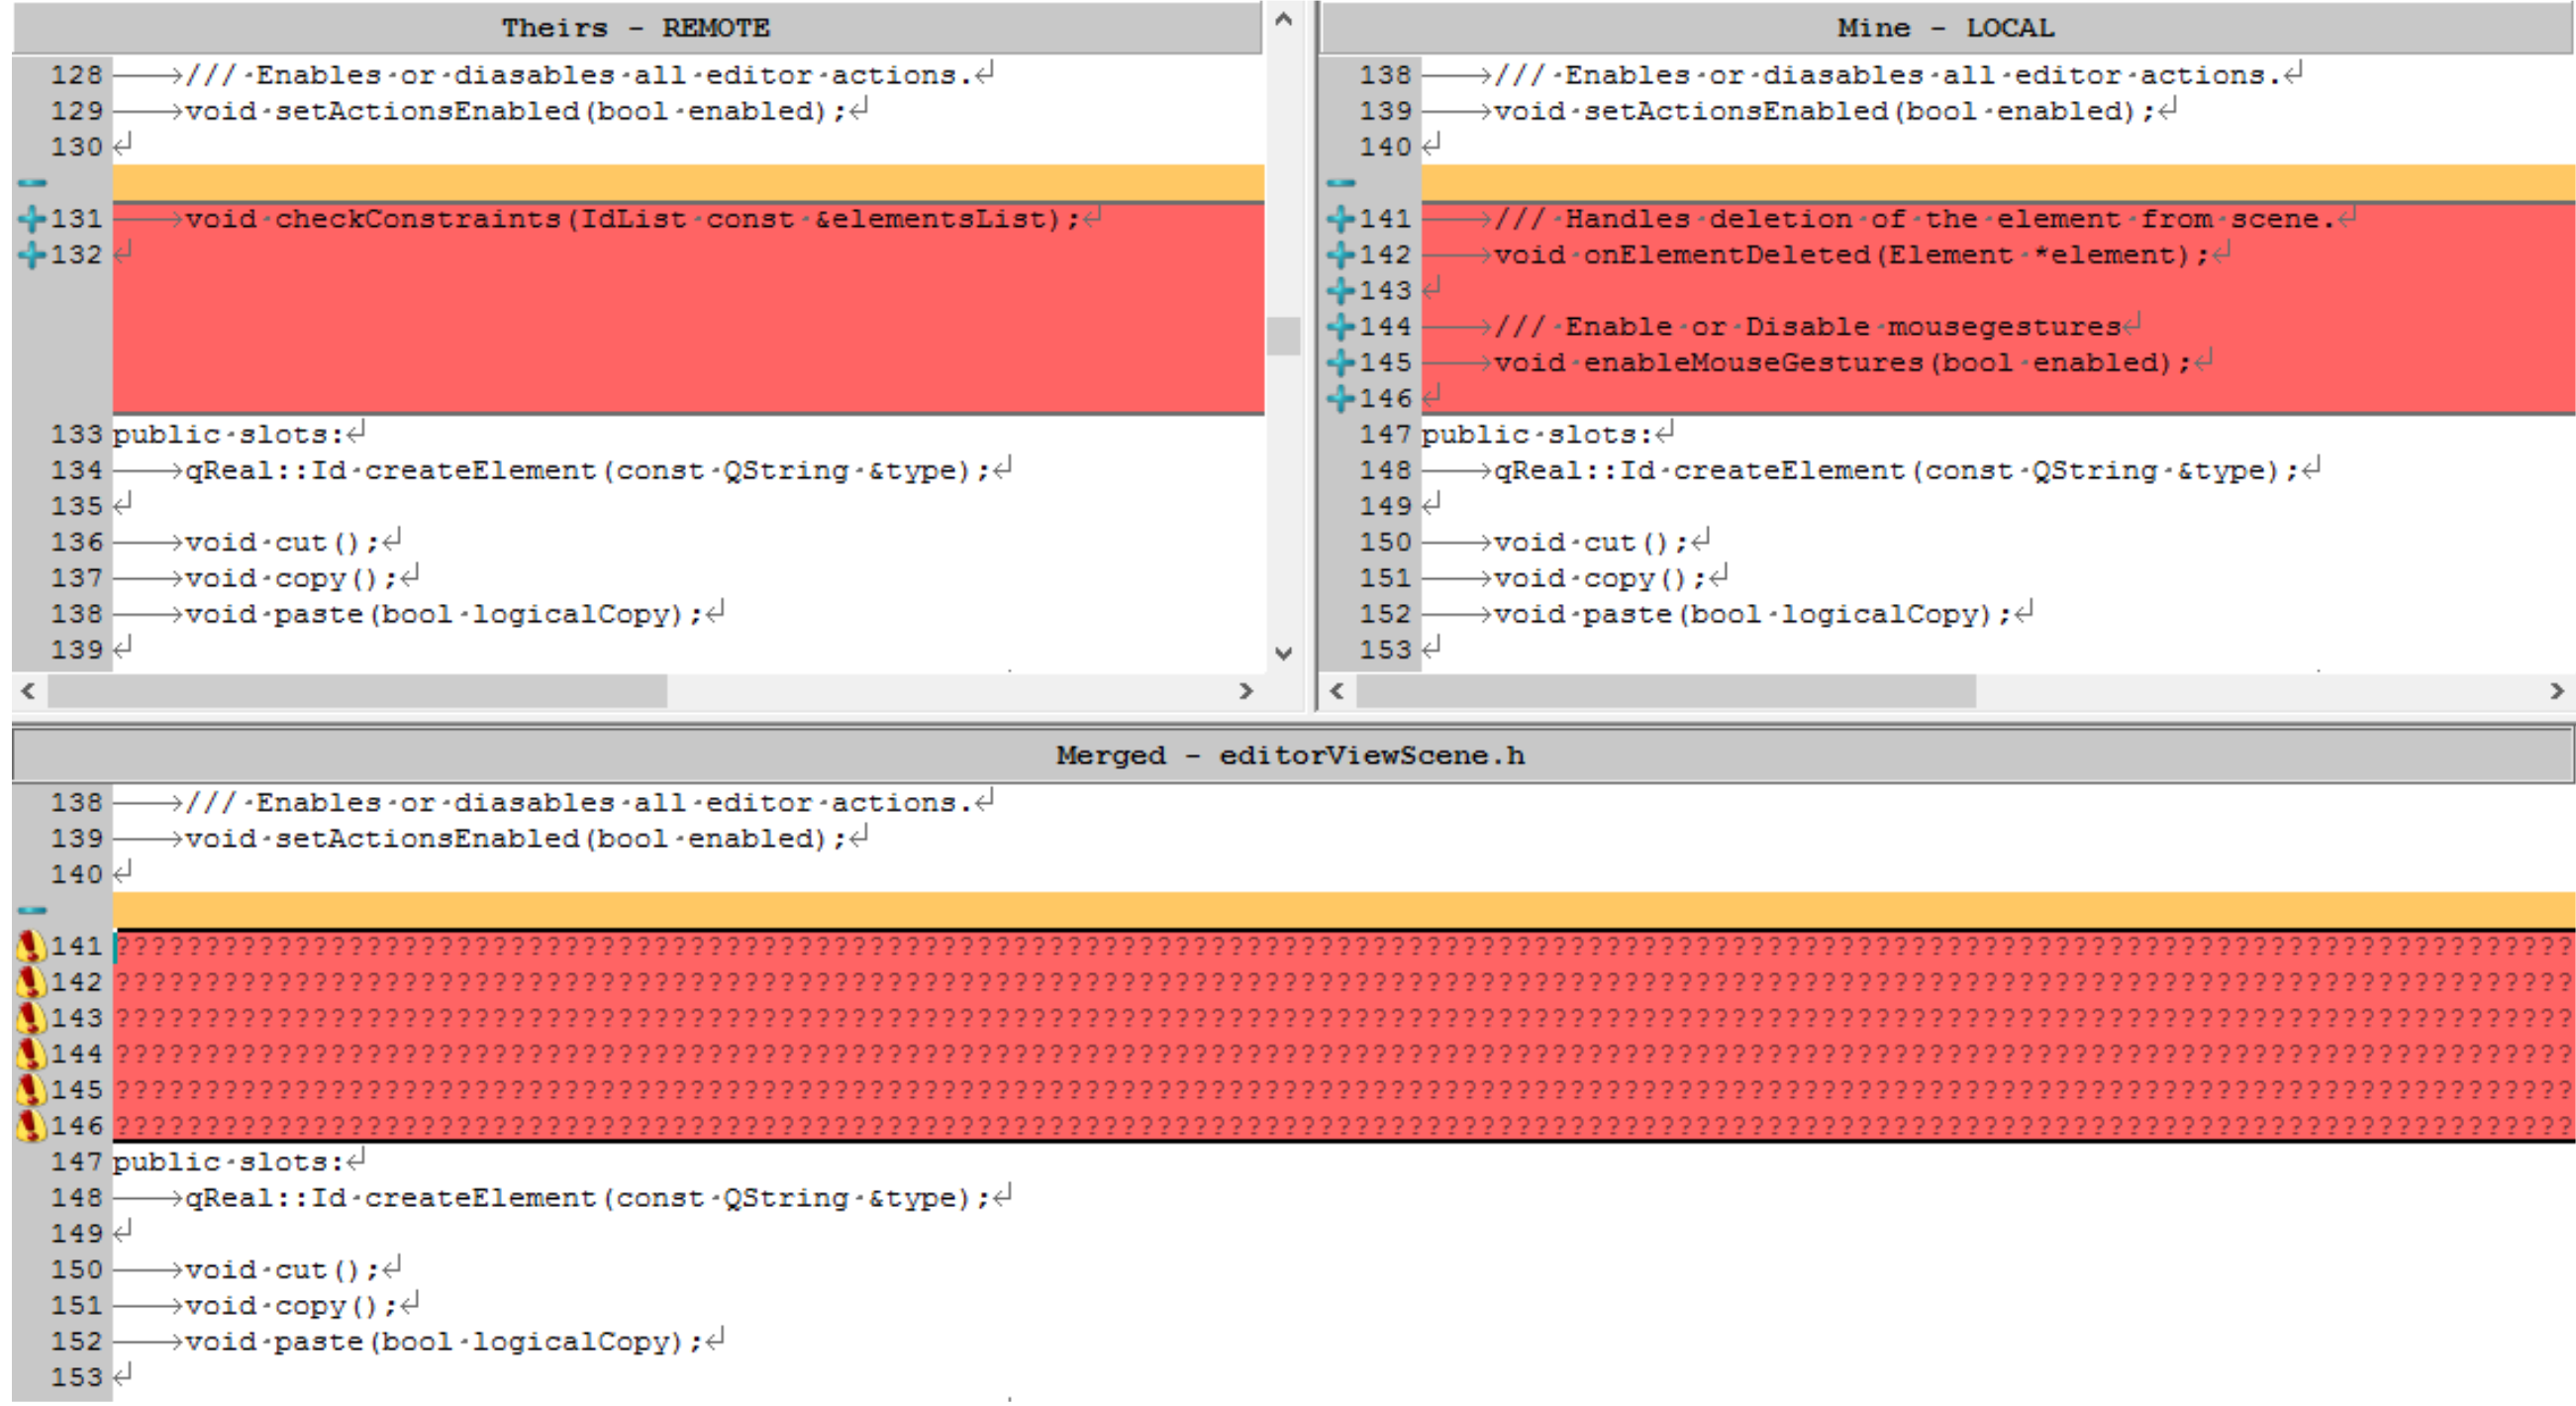
\includegraphics[width=0.95\textwidth]{conflicts.png}
		\end{center}
	\end{frame}

	\begin{frame}
		\frametitle{Конфликты в коде}
		\begin{center}
			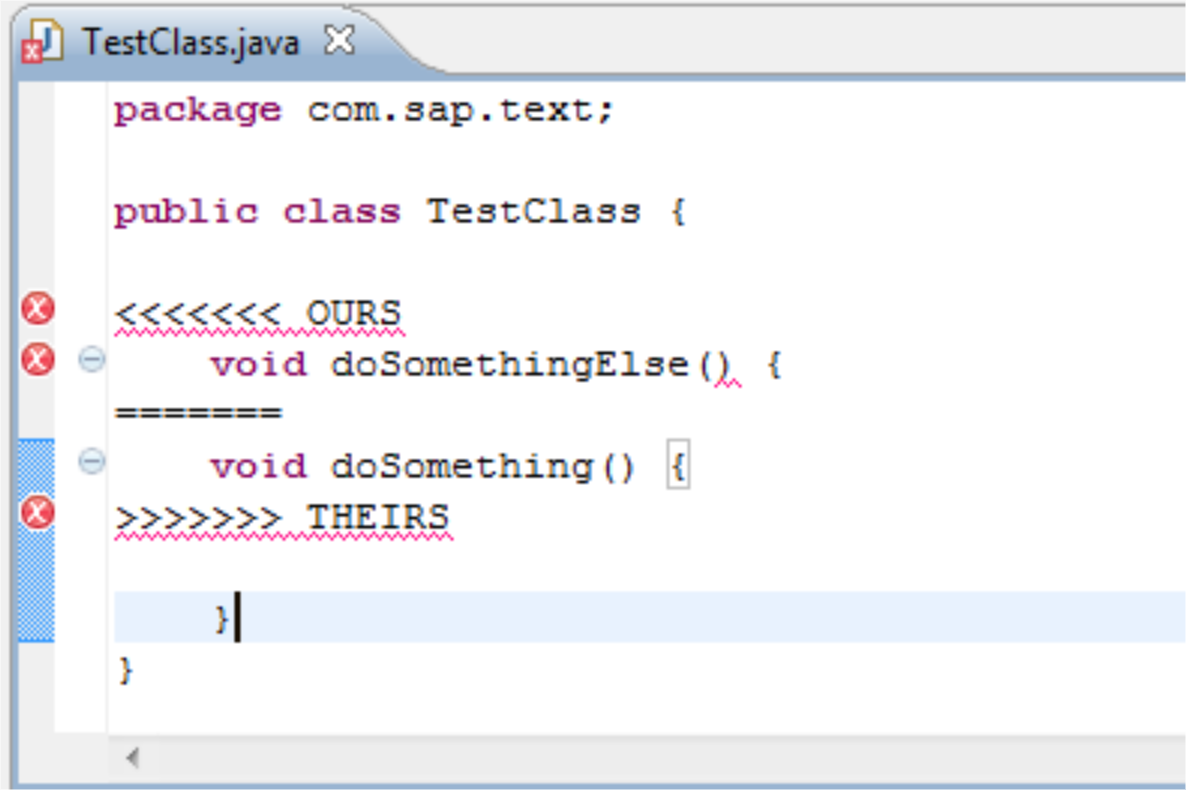
\includegraphics[width=0.5\textwidth]{conflictsInCode.png}
		\end{center}
	\end{frame}

	\begin{frame}[fragile]
		\frametitle{Rebase}
		\begin{minted}{text}
$ git checkout experiment
$ git rebase master
First, rewinding head to replay your work on top of it...
Applying: added staged command
		\end{minted}
		\begin{center}
			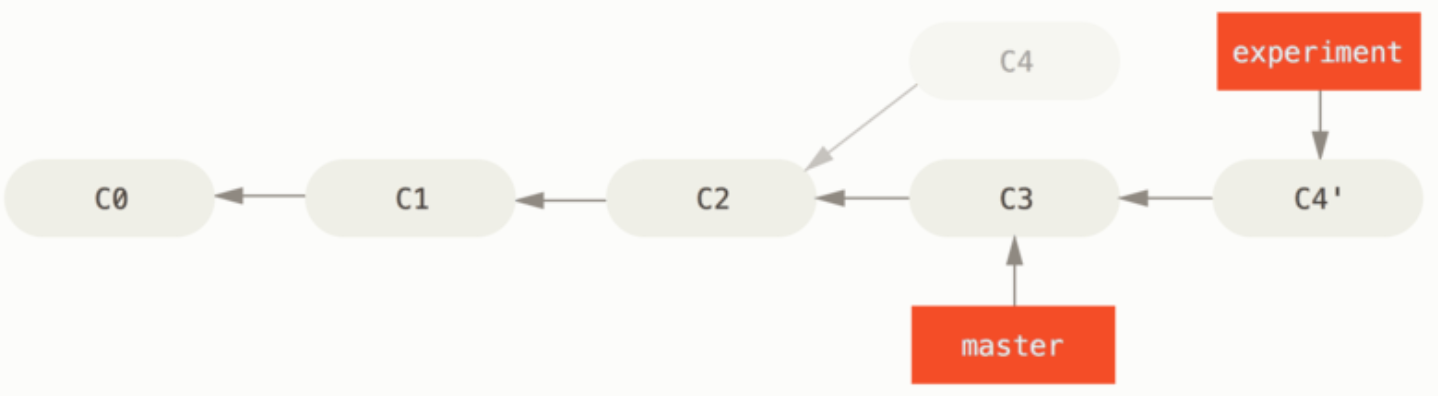
\includegraphics[width=0.8\textwidth]{rebase.png}
			\attribution{https://git-scm.com/book/ru}
		\end{center}
	\end{frame}

	\section{Тэги}

	\begin{frame}[fragile]
		\frametitle{Тэги}
		Последний из объектов в Git --- tag. Это просто указатель на коммит.
		\begin{footnotesize}
			\begin{itemize}
				\item Легковесный тэг:
					\begin{minted}{text}
git update-ref refs/tags/v1.0 cac0cab538b970a37ea1e769cbbde608743bc96d
					\end{minted}
					Или просто git tag
				\item Аннотированный тэг:
					\begin{minted}{text}
$ git tag -a v1.1 1a410efbd13591db07496601ebc7a059dd55cfe9 -m 'test tag'

$ git cat-file -p 9585191f37f7b0fb9444f35a9bf50de191beadc2
object 1a410efbd13591db07496601ebc7a059dd55cfe9
type commit
tag v1.1
tagger Scott Chacon <schacon@gmail.com> Sat May 23 16:48:58 2009 -0700

test tag
					\end{minted}
			\end{itemize}
		\end{footnotesize}
	\end{frame}

	\section{Packfiles}

	\begin{frame}[fragile]
		\frametitle{Packfiles}
		Пока что получалось, что все версии всех файлов в Git хранятся целиком, как они есть. Все они сжимаются zlib, но в целом, если создать репозиторий, добавлять туда файлы, коммитить и т.д., все версии всех файлов будут в нём целиком. На помощь приходят .pack-файлы:
		\begin{center}
			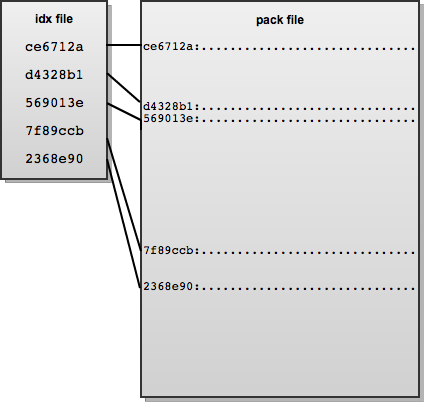
\includegraphics[width=0.4\textwidth]{gitPackFiles.png}
		\end{center}
	\end{frame}

	\section{Хорошие практики}

	\begin{frame}
		\frametitle{Хорошие практики}
		\begin{itemize}
			\item Коммитим только исходные тексты, конфиги, картинки и т.п.
			\item Если что-то может быть автоматически сгенерировано по тому, что уже есть в репозитории, это НЕ коммитим
			\item Всегда пишем адекватные комментарии к коммитам
			\begin{itemize}
				\item Одно-два осмысленных предложения
				\item За комментарии типа ``fix'' придётся освоить искусство отката веток (или хотя бы amend)
			\end{itemize}
			\item Коммитим как можно чаще
			\begin{itemize}
				\item Сделали что-то осмысленное --- коммит
			\end{itemize}
		\end{itemize}
	\end{frame}

	\begin{frame}
		\frametitle{Хорошие практики (2)}
		\begin{itemize}
			\item Коммит не должен содержать в себе файлы, не относящиеся к изменениям
			\begin{itemize}
				\item .gitignore
				\item Обязательно надо проверять, что коммитим
			\end{itemize}
			\item Коммит не должен добавлять/убирать пустые строки, менять пробелы на табы и т.д., если это не суть коммита
			\item Стиль исходного кода и отступов должен совпадать с текстом вокруг
			\item Делаете пуллреквест --- посмотрите diff
		\end{itemize}
		\begin{center}
			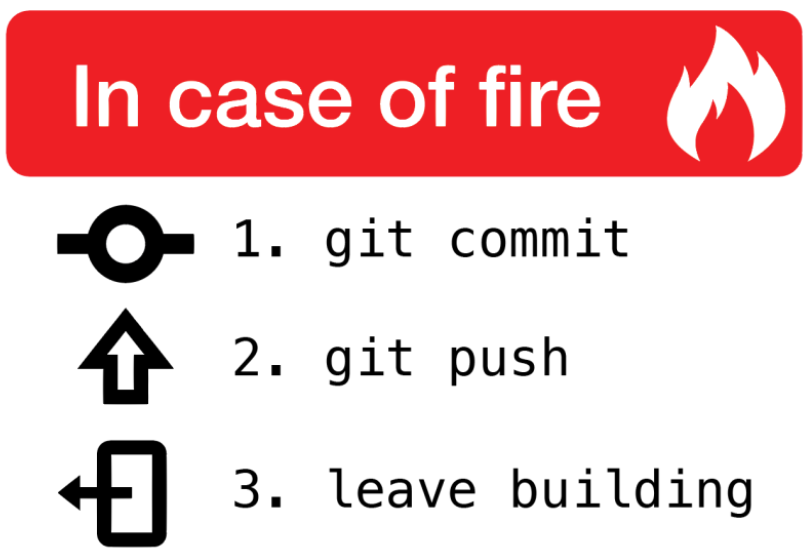
\includegraphics[width=0.4\textwidth]{inCaseOfFire.png}
		\end{center}
	\end{frame}

	\begin{frame}
		\frametitle{Git Flow}
		\begin{center}
			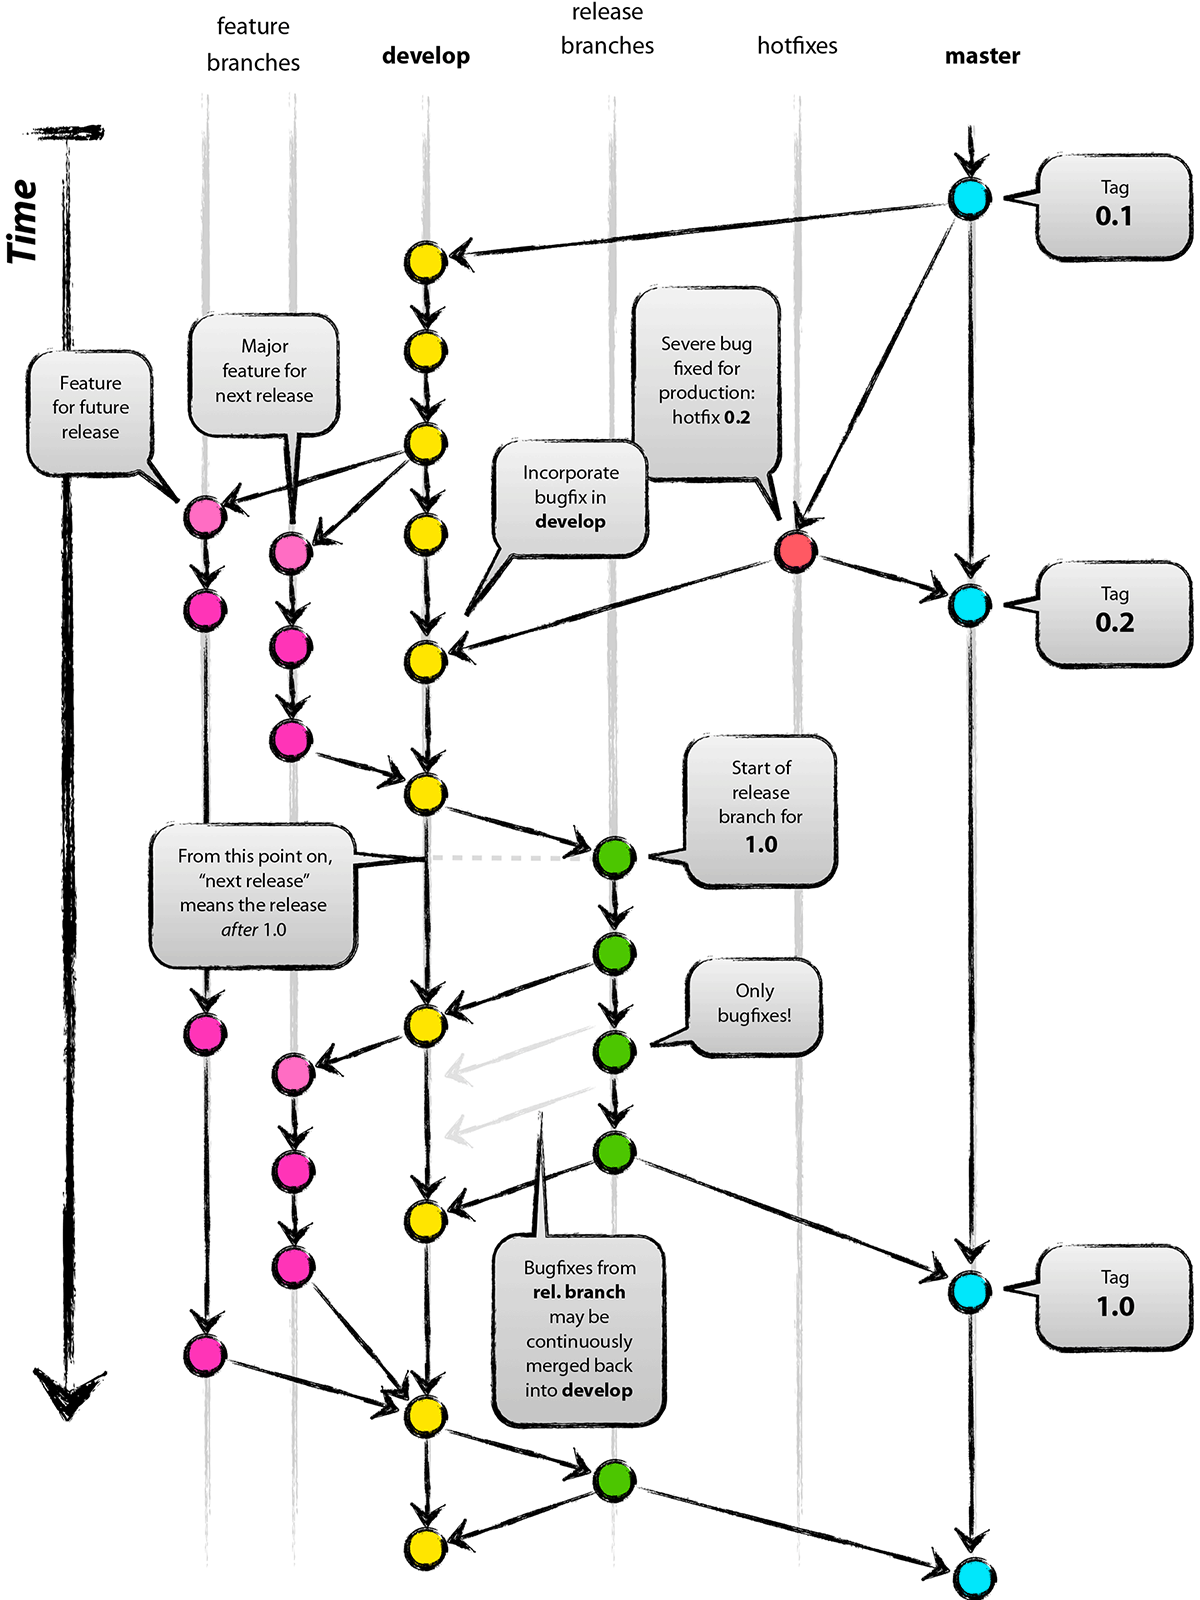
\includegraphics[width=0.42\textwidth]{gitFlow.png}
			\attribution{https://nvie.com/posts/a-successful-git-branching-model/}
		\end{center}
	\end{frame}

	\begin{frame}[fragile]
		\frametitle{Ещё полезные команды}
		\begin{itemize}
			\item \verb|git add -p| --- интерактивное добавление изменений к коммиту, позволяет коммитить только часть файла
			\item \verb|git commit --amend| --- исправить последний коммит
			\begin{itemize}
				\item \verb|git commit --amend -m "an updated commit message"|
				\item Применять \textbf{только до} git push
			\end{itemize}
			\item \verb|git reset --hard| --- откатить все изменения в рабочей копии до последнего коммита
			\begin{itemize}
				\item Обязательно проверить git status, что не откатите лишнего
			\end{itemize}
			\item \verb|git reset --hard <хеш коммита>| --- откатить все изменения в текущей ветке до указанного коммита, забыть все коммиты, что были после
			\begin{itemize}
				\item И случайно грохнуть всю домашку перед зачётом
			\end{itemize}
		\end{itemize}
	\end{frame}

	\section{.gitignore}

	\begin{frame}
		\frametitle{.gitignore}
		\begin{itemize}
			\item Локальный для репозитория и глобальный
			\item Glob-шаблоны
			\item \# --- комментарий
			\item Можно заканчивать шаблон символом / для указания каталога
			\item можно инвертировать шаблон, использовав ! в качестве первого символа
			\item Glob
			\begin{itemize}
				\item \mintinline{text}|*| --- 0 или более символов
				\item \mintinline{text}|?| --- один символ
				\item \mintinline{text}|[abc]| --- любой символ из указанных в скобках
				\item \mintinline{text}|[0-9]| --- любой символ из интервала
			\end{itemize}
		\end{itemize}
	\end{frame}

	\begin{frame}[fragile]
		\frametitle{Пример}
		\begin{minted}{bash}
# не обрабатывать файлы, имя которых заканчивается на .a
*.a
# НО отслеживать файл lib.a, несмотря на то, что мы игнорируем все .a файлы 
!lib.a
# игнорировать только файл TODO, находящийся в корневом каталоге
/TODO
# игнорировать все файлы в каталоге build/
build/
# игнорировать doc/notes.txt, но не doc/server/arch.txt
doc/*.txt
# игнорировать все .txt файлы в каталоге doc/
doc/**/*.txt
		\end{minted}
		\begin{itemize}
			\item \url{https://github.com/github/gitignore}
		\end{itemize}
	\end{frame}

\end{document}
